\documentclass{article}

\usepackage{graphicx}
\usepackage{rotating}
\usepackage{amsmath}
\usepackage{amssymb}
\usepackage{fancyhdr}
\usepackage{listings}
%\usepackage{xcolor}
\usepackage{longtable}
\usepackage{color}
\usepackage{amsfonts}
\usepackage{textcomp}
\usepackage{float}
\usepackage[sorting=none]{biblatex}
\usepackage[margin=1in]{geometry}
\usepackage[font={small,it}]{caption}
\usepackage[table,xcdraw]{xcolor}
\usepackage{placeins}
\usepackage{xepersian}





%\DeclareMathOperator*{\btie}{\bowtie}
\addbibresource{bibliography.bib}
\settextfont[Scale=1.2]{B-NAZANIN.TTF}
\setlatintextfont[Scale=1]{Times New Roman}
\renewcommand{\baselinestretch}{1.5}
\pagestyle{fancy}
\fancyhf{}
\rhead{تکلیف دوم درس مبانی رمزنگاری}
\lhead{\thepage}
\rfoot{علیرضا ابره فروش}
\lfoot{9816603}
\renewcommand{\headrulewidth}{1pt}
\renewcommand{\footrulewidth}{1pt}
%%%%%%%%%%
\lstset
{
    language=[latex]tex,
    basicstyle=\ttfamily,
    commentstyle=\color{black},
    columns=fullflexible,
    keepspaces=true,
    upquote=true,
    showstringspaces=false,
    morestring=[s]\\\%,
    stringstyle=\color{black},
}
%%%%%%%%%%
%beginMatlab
\definecolor{mygreen}{RGB}{28,172,0} % color values Red, Green, Blue
\definecolor{mylilas}{RGB}{170,55,241}
%endMatlab
\begin{document}
%beginMatlab
\lstset{language=Matlab,%
    %basicstyle=\color{red},
    breaklines=true,%
    morekeywords={matlab2tikz},
    keywordstyle=\color{blue},%
    morekeywords=[2]{1}, keywordstyle=[2]{\color{black}},
    identifierstyle=\color{black},%
    stringstyle=\color{mylilas},
    commentstyle=\color{mygreen},%
    showstringspaces=false,%without this there will be a symbol in the places where there is a space
    numbers=left,%
    numberstyle={\tiny \color{black}},% size of the numbers
    numbersep=9pt, % this defines how far the numbers are from the text
    emph=[1]{for,end,break},emphstyle=[1]\color{red}, %some words to emphasise
    %emph=[2]{word1,word2}, emphstyle=[2]{style},    
}
%endMatlab
\begin{titlepage}
\begin{center}

\includegraphics[width=0.4\textwidth]{figures/IUT Logo.png}\\
        
\LARGE
\textbf{دانشگاه صنعتی اصفهان}\\
\textbf{دانشکده مهندسی برق و کامپیوتر}\\
        
\vfill
        
\huge
\textbf{عنوان: تکلیف چهارم درس ریزپردازنده}\\
        
\vfill
        
\LARGE
\textbf{نام و نام خانوادگی: علیرضا ابره فروش}\\
\textbf{شماره دانشجویی: 9816603}\\
\textbf{نیم\,سال تحصیلی: پاییز 1400}\\
\textbf{مدرّس: دکتر عارف کریمی افشار}\\
\end{center}
\end{titlepage}


%\tableofcontents
\newpage


\section{}%1
\begin{latin}
"One-time pad is a cryptographic encryption technique that uses a random key that is as long as the message itself. The key is used only once, and both the sender and receiver must have a copy of the same key to encrypt and decrypt messages. Here are some pros and cons of one-time pad:\\
Pros:
\begin{enumerate}

    \item Security: One-time pad encryption is considered to be unbreakable if used correctly, as it provides perfect secrecy. The encryption key used is completely random and cannot be guessed or predicted, making it virtually impossible for an attacker to break.

    \item Simplicity: One-time pad encryption is simple to understand and implement, as it involves only the use of a random key and the XOR operation. It does not require complex algorithms or mathematical computations, making it a preferred choice for encrypting short messages.

    \item Privacy: One-time pad encryption ensures complete privacy, as it does not reveal any information about the original message, even if an attacker intercepts the ciphertext.
\end{enumerate}
Cons:
\begin{enumerate}
    \item Key distribution: One-time pad encryption requires both the sender and the receiver to have a copy of the same key. This can be challenging in practice, especially if the keys need to be distributed securely over long distances.

    \item Key management: The one-time pad key can be used only once and must be discarded after use, making key management a challenge. Generating a truly random key that is as long as the message itself can also be difficult.

    \item Size limitations: One-time pad encryption requires a key that is as long as the message, which can make it impractical for encrypting large amounts of data.

    \item Vulnerable to certain attacks: One-time pad encryption is vulnerable to certain attacks, such as key reuse or guessing attacks, which can compromise the security of the encryption."
\end{enumerate}
\end{latin}

\section{}%2
\subsection{}
\begin{latin}
\begin{enumerate}
\item LFSRs which generate a maximum-length sequence. These LFSRs are based on
primitive polynomials.
\item LFSRs which do not generate a maximum-length sequence but whose sequence
length is independent of the initial value of the register. These LFSRs are based
on irreducible polynomials that are not primitive. Note that all primitive polynomials are also irreducible.
\item LFSRs which do not generate a maximum-length sequence and whose sequence
length depends on the initial values of the register. These LFSRs are based on
reducible polynomials.
\end{enumerate}
\end{latin}

\subsection{}
\subsubsection{}
\begin{latin}
$
P\left( x \right) = x ^ 4 + x ^ 3 + x ^ 2 + x + 1\\
m = 4\\
p_3 = p_2 = p_1 = p_0 = 1
$
\end{latin}
\begin{figure}[H]
    \centering
    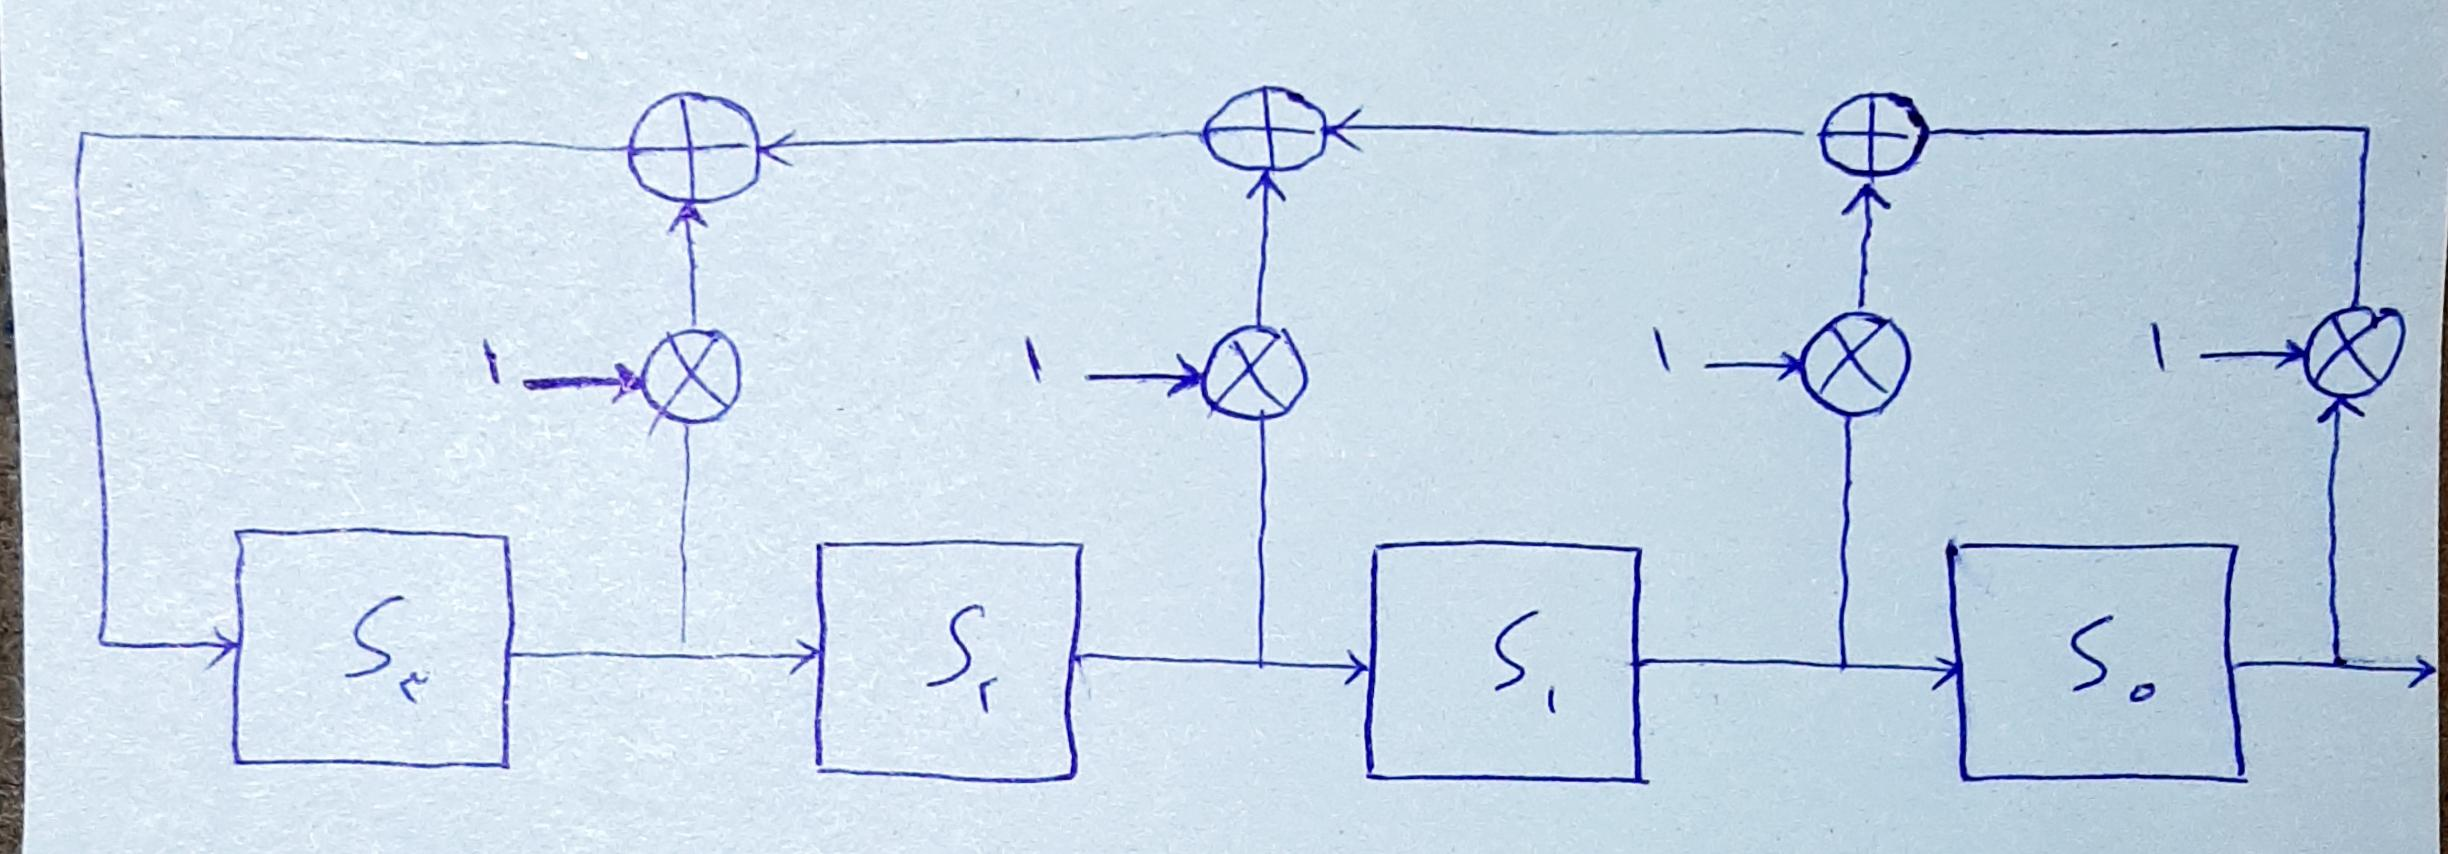
\includegraphics[width=0.75\textwidth]{figures/1.jpg}
    \caption
	{}
    \label{fig:fig1}
\end{figure}
از آنجایی که این چندجمله‌ای را نمی‌توان به چندجمله‌ای غیر 1ای تجزیه کرد پس \lr{irreducible} است. پس این \lr{LFSR} \lr{reducible} نیست. برای بررسی اینکه آیا \lr{primitive} است باید بررسی کنیم که آیا طول بزرگترین دنباله‌ای که تولید می‌کند ماکسیمم ($2^4 - 1$) هست یا نه. طبق جدول زیر تناوب طولانی‌ترین دنباله ساخته شده توسط این \lr{LFSR} برابر 5 است که کمتر از 15 است. پس این \lr{LFSR} \lr{primitive} نیست. در نتیجه این \lr{LFSR}  بر پایه‌ی \lr{primitive polynomial} است.
\begin{latin}
% Please add the following required packages to your document preamble:
% \usepackage{longtable}
% Note: It may be necessary to compile the document several times to get a multi-page table to line up properly
\begin{longtable}[c]{l|c|c|c|c|}
\cline{2-5}
1 & 0 & 1 & 0 & 1          \\ \cline{2-5} 
\endfirsthead
%
\endhead
%
2 & 0 & 0 & 1 & 0          \\ \cline{2-5} 
3 & 1 & 0 & 0 & 1          \\ \cline{2-5} 
4 & 0 & 1 & 0 & \textbf{0} \\ \cline{2-5} 
5 & 1 & 0 & 1 & 0          \\ \cline{2-5} 
6 & 0 & 1 & 0 & 1          \\ \cline{2-5} 
\end{longtable}
\end{latin}

\subsubsection{}
\begin{latin}
$
P\left( x \right) = x ^ 3 + x + 1\\
m = 3\\
p_2 = 0,  p_1 = p_0 = 1
$
\end{latin}
\begin{figure}[H]
    \centering
    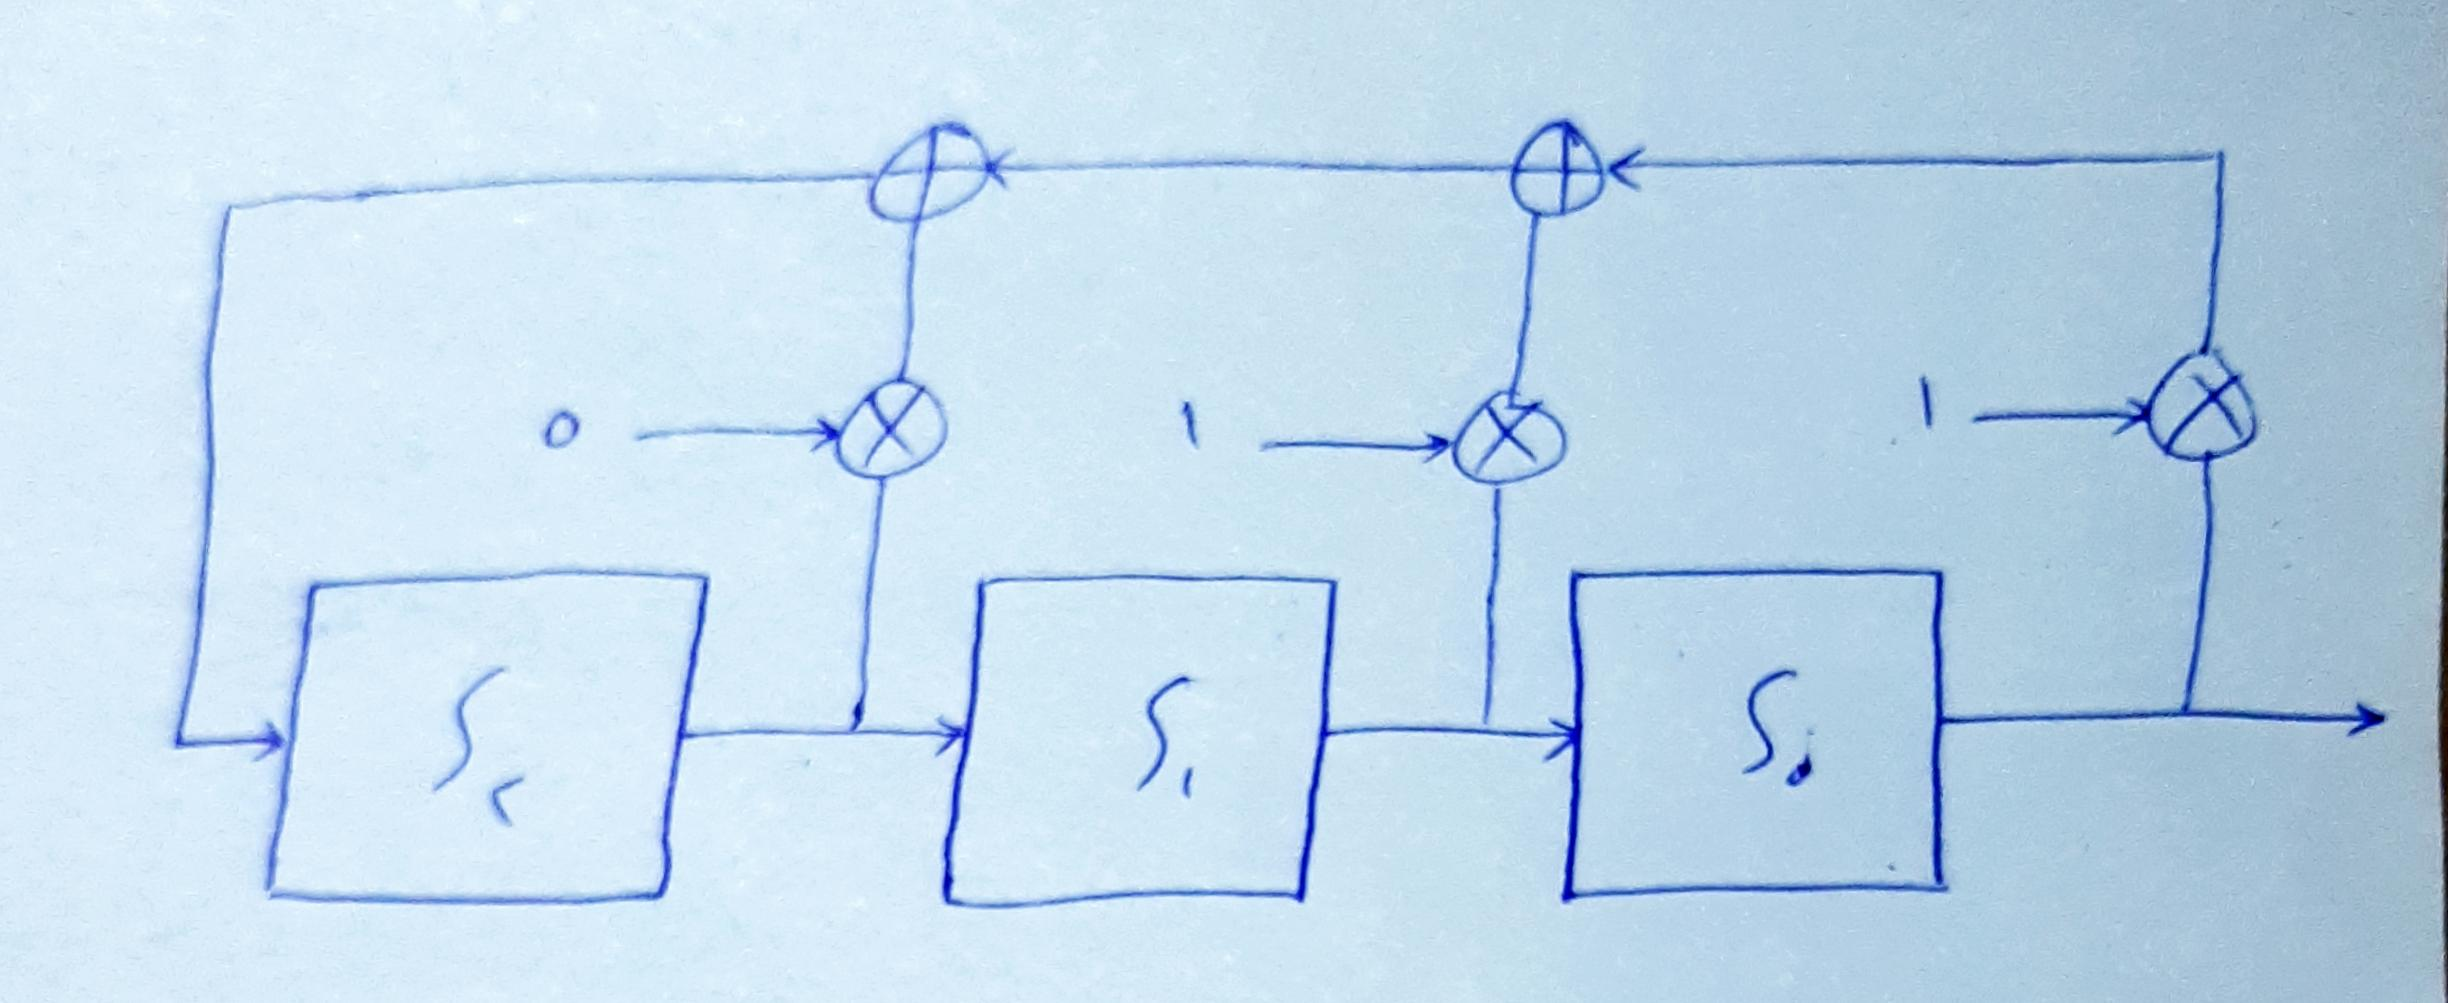
\includegraphics[width=0.75\textwidth]{figures/2.jpg}
    \caption
	{}
    \label{fig:fig1}
\end{figure}
از آنجایی که این چندجمله‌ای را نمی‌توان به چندجمله‌ای غیر 1ای تجزیه کرد پس \lr{irreducible} است. پس این \lr{LFSR} \lr{reducible} نیست. برای بررسی اینکه آیا \lr{primitive} است باید بررسی کنیم که آیا طول بزرگترین دنباله‌ای که تولید می‌کند ماکسیمم ($2^3 - 1$) هست یا نه. طبق جدول زیر تناوب طولانی‌ترین دنباله ساخته شده توسط این \lr{LFSR} برابر 7 است. پس این \lr{LFSR} \lr{primitive} است.
\begin{latin}
% Please add the following required packages to your document preamble:
% \usepackage{longtable}
% Note: It may be necessary to compile the document several times to get a multi-page table to line up properly
\begin{longtable}[c]{c|c|c|c|}
\cline{2-4}
1 & 1 & 0 & 1          \\ \cline{2-4} 
\endfirsthead
%
\endhead
%
2 & 1 & 1 & 0          \\ \cline{2-4} 
3 & 1 & 1 & 1          \\ \cline{2-4} 
4 & 0 & 1 & \textbf{1} \\ \cline{2-4} 
5 & 0 & 0 & 1          \\ \cline{2-4} 
6 & 1 & 0 & 0          \\ \cline{2-4} 
7 & 0 & 1 & 0          \\ \cline{2-4} 
8 & 1 & 0 & 1          \\ \cline{2-4} 
\end{longtable}
\end{latin}



\section{}%3

\begin{latin}
$
y_i \equiv x_i + s_i \quad mod\:2 \\ \Rightarrow 
s_i \equiv y_i - x_i \equiv y_i + x_i \quad mod\:2 \\ \Rightarrow 
$
% Please add the following required packages to your document preamble:
% \usepackage{longtable}
% Note: It may be necessary to compile the document several times to get a multi-page table to line up properly
\begin{longtable}[c]{c|c|c|c|c|c|c|c|c|c|c|c|c|c|c|c|c|c|c|c|c|c|c|c|c|c|c|c|c|}
\cline{2-29}
$x_i$ & 1 & 0 & 0 & 1 & 0 & 0 & 1 & 0 & 0 & 1 & 1 & 0 & 1 & 1 & 0 & 1 & 1 & 0 & 0 & 1 & 0 & 0 & 1 & 0 & 0 & 1 & 1 & 0 \\ \cline{2-29} 
\endfirsthead
%
\endhead
%
$y_i$ & 1 & 0 & 1 & 1 & 1 & 1 & 0 & 0 & 0 & 0 & 1 & 1 & 0 & 0 & 0 & 1 & 0 & 0 & 1 & 0 & 1 & 0 & 1 & 1 & 0 & 0 & 0 & 1 \\ \cline{2-29} 
$s_i$ & 0 & 0 & 1 & 0 & 1 & 1 & 1 & 0 & 0 & 1 & 0 & 1 & 1 & 1 & 0 & 0 & 1 & 0 & 1 & 1 & 1 & 0 & 0 & 1 & 0 & 1 & 1 & 1 \\ \cline{2-29} 
\end{longtable}
\end{latin}

\subsection{}
با فرض \lr{primitive} بودن \lr{LFSR}ِ، و با توجه به اینکه دنباله‌ی به طول هفتِ 0010111 چهار بار تکرار شده است، احتمالا \lr{LFSR} تولید کننده‌ی این \lr{key stream} از درجه‌ی $\log_2 \left( 7 + 1 \right) = 3$ است.

\subsection{}
مقدار اولیه‌ی \lr{LFSR} با توجه به قسمت قبل برابر سه بیت اول دنباله است که برابر است با 001.

\subsection{}
\begin{latin}
$
\begin{bmatrix}
s_2 & s_1 & s_0 \\
s_3 & s_2 & s_1 \\
s_4 & s_3 & s_2
\end{bmatrix}
\begin{bmatrix}
p_2 \\
p_1 \\
p_0
\end{bmatrix}=
\begin{bmatrix}
s_3 \\
s_4 \\
s_5
\end{bmatrix}=
\begin{bmatrix}
0 \\
1 \\
1
\end{bmatrix} \\ \Rightarrow
\begin{bmatrix}
s_2 & s_1 & s_0 \\
s_3 & s_2 & s_1 \\
s_4 & s_3 & s_2
\end{bmatrix}^{-1}=
\begin{bmatrix}
1 & 0 & 0 \\
0 & 1 & 0 \\
0 & 0 & 1
\end{bmatrix} \\ \Rightarrow
\begin{bmatrix}
p_2 \\
p_1 \\
p_0
\end{bmatrix}=
\begin{bmatrix}
1 & 0 & 0 \\
0 & 1 & 0 \\
0 & 0 & 1
\end{bmatrix}
\begin{bmatrix}
0 \\
1 \\
1
\end{bmatrix}=
\begin{bmatrix}
0 \\
1 \\
1
\end{bmatrix}
$
\end{latin}

\subsection{}
\begin{figure}[H]
    \centering
    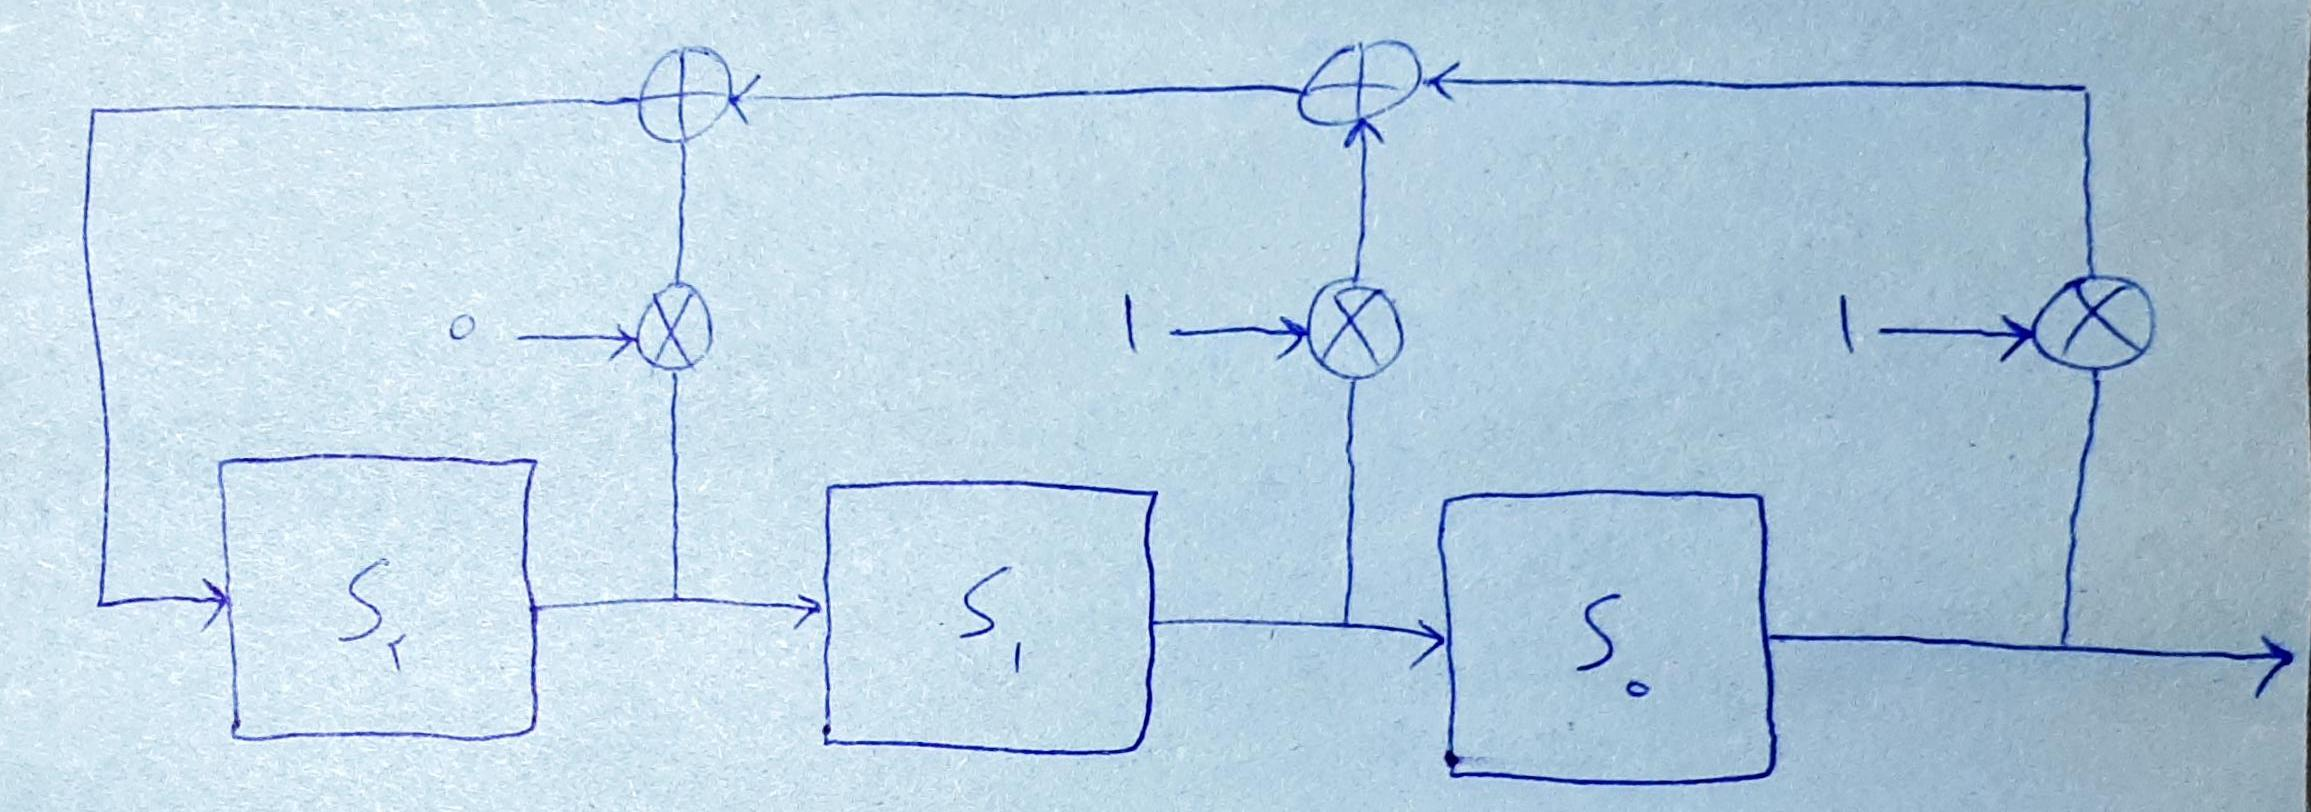
\includegraphics[width=0.75\textwidth]{figures/3.jpg}
    \caption
	{}
    \label{fig:fig1}
\end{figure}

\begin{latin}
$
s_{i+1} \equiv s_{i-2} + s_{i-3} \quad mod\:2
$
% Please add the following required packages to your document preamble:
% \usepackage{longtable}
% Note: It may be necessary to compile the document several times to get a multi-page table to line up properly
\begin{longtable}[c]{c|c|c|c|}
\cline{2-4}
1 & 1 & 0 & 0 \\ \cline{2-4}
\endfirsthead
%
\endhead
%
2 & 0 & 1 & 0 \\ \cline{2-4} 
3 & 1 & 0 & 1 \\ \cline{2-4} 
4 & 1 & 1 & 0 \\ \cline{2-4} 
5 & 1 & 1 & 1 \\ \cline{2-4} 
6 & 0 & 1 & 1 \\ \cline{2-4} 
7 & 0 & 0 & 1 \\ \cline{2-4} 
8 & 1 & 0 & 0 \\ \cline{2-4} 
\end{longtable}
\end{latin}
با توجه به جدول بالا درست است.


\section{}%4




\section{}%5




%------------------------------------------------------------------------------------------


\subsection*{منابع}



\end{document}
